\documentclass{article}
\usepackage[utf8]{inputenc}
\usepackage{graphicx}
\usepackage{float}

\title{Augmented Chess (WE)}
\author{jmorte14, marand13, tmccol14}
\date{September 2017}

\begin{document}

\maketitle

\section{Description}
Our project entails the development of an online game. The game is inspired by "Stratego" and "Chess" among others. It is turn based with one army of pieces facing another on a board with 8x8 fields. Armies are created beforehand and players queue up using a similar amount of points to spend on army creation. The objective of the game is to defeat the enemy king.

The game supports persistent armies, meaning that players may store created armies for later use. The system allows players to queue up with a army and be matched up against another player with an army in the same bracket.

\section{Requirements}
\textbf{Must have}
\begin{itemize}
    \item Users can register accounts
    \item Users can log in to their account
    \item Users can create and edit an army
    \item When a user creates an army, the units may be purchased or upgraded with Army points (Users are matched against armies with similar points spend, e.g. under 100 points spend)
    \item Users can play Augmented Chess against other players with a selected army on a single client
\end{itemize}
\textbf{Nice to have}
\begin{itemize}
    \item Play games against users on other clients
    \item Users can compete for a spot on a leaderboard
\end{itemize}

\section{Data model}
The data model was developed in WebRatio and can be seen in figure \ref{fig:data-model}. The model consists for eight entities, \texttt{User, Queue, Game, Army, Board, turnLog, Piece}. The \texttt{User} entity represents the user and stores a user-name. The user-name is used as log-in credentials, this is not secure, but the system holds no sensitive information what so ever. Armies consists of pieces which represent the usual chess pieces, but with additional stats that can be modified using army points. The queue and the game entities keep track of users wating to join a game and users playing a game. The \texttt{turnLog} represents the events of a turn. Finally during a game, the \texttt{Board} and \texttt{Cell} entities keep track of the game state. A \texttt{Cell} may contain up to one \texttt{Piece}, since the \texttt{Cells} are part of the \texttt{Board} it can track the game progress.
\begin{figure}[H]
    \centering
    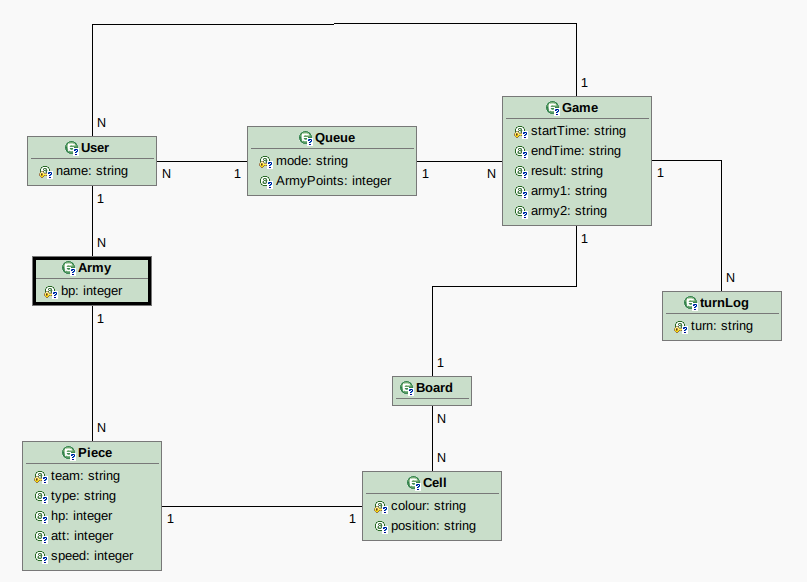
\includegraphics[width=\textwidth]{data-model.png}
    \caption{Data model}
    \label{fig:data-model}
\end{figure}

\section{Hypertext model}
The hypertext model can be see in figure \ref{fig:hypertext-model}. It contains four areas \texttt{Main}, \texttt{Army Creater}, \texttt{Queue} and \texttt{In-game}. These all contain multiple pages responsible for different aspects of the web site.

When using the web site the user starts by logging in from the \textit{Login} screen, or navigating directly to the \textit{Menu} screen by url. If the user is not registered, this can be done by navigating to the \textit{Register} screen from the login screen. From the menu screen the user can either navigate to the \textit{Army Creator} screen and create or edit an army or navigate to the \textit{Queue} screen, where the user can start searching for a game. Once a game is found, the user is sent to the \textit{In-game}, where the game can take place.

\begin{figure}[H]
    \centering
    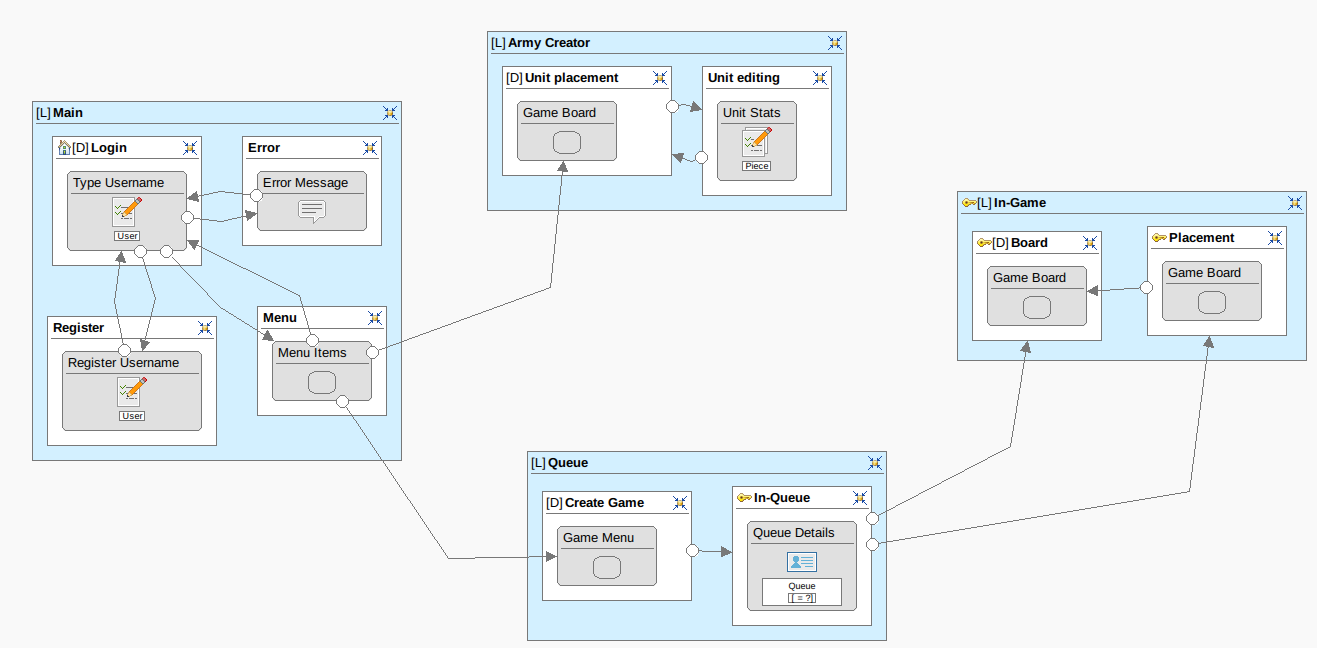
\includegraphics[width=\textwidth]{hypertext-model.png}
    \caption{Hypertext model}
    \label{fig:hypertext-model}
\end{figure}

\end{document}
